\documentclass[letterpaper, twocolumn]{article}
\pagestyle{plain}

\usepackage[margin=2.5cm]{geometry}
\usepackage{multicol}
\usepackage{url}
\usepackage{graphicx}

\title{CMSC818s: Project 3 \\
A Brief Survey of Modern Virtualization Research}
\author{}
\date{}

\begin{document}

\twocolumn[
\begin{@twocolumnfalse}
\maketitle

\vspace{-2cm}

\begin{center}
\begin{multicols}{2}
  Greg Benjamin \\
  gregben@cs.umd.edu \\
  Austin Myers \\
  amyers@cs.umd.edu
\end{multicols}
Department of Computer Science \\
University of Maryland, College Park
\end{center}

\end{@twocolumnfalse}
]

\section{Introduction}
\label{sec:intro}

The concept of virtualization has been around for a long time, reaching back
to the 1960s and the introduction of virtual memory in timeshared machines.
However, in the last decade or so it's become a very exciting area of research,
particularly motivated by a new market for server virtualization.  Commerical
products like VMWare and open-source platforms like Xen \cite{ref:xen} have made
it possible for companies to host dozens of instances of their servers
on the same hardware.  Companies can now spend less on metal, can seamlessly and
easily migrate servers from one machine to another, and can even vary their fleet
size on the fly in response to fluctuations in server traffic by spinning up new
instances.  In addition to the commercial successes that have come as a result
of server virtualization, there have been tremendous breakthroughs in the research
community as well, ranging from new solutions to problems of isolation and protection
to novel new algorithms for scheduling and resource allocation.

Despite the flurry of interest in this area, there are still many interesting
and difficult problems to be solved.  Sharing finite resources
fairly and safely amongst many competing processes has never been easy, but
the popularity of virtualization in the cloud makes scalability and efficiency
bigger concerns than ever before.  Furthermore, the commercialization of
virtual machines raises questions of how to ensure quality of service in
an environment where everyone is in contention for the hardware.  In this
paper, we will examine some of the recent literature in this area and
seek to draw some conclusions about the problem space and the directions
of future work.

The rest of the paper is structured as follows: in Section \ref{sec:background}
we provide background information on the history of virtualization and the
sorts of techniques which are utilized today.  Section \ref{sec:summaries}
presents summaries of a foundation virtualization paper from the
5\textsuperscript{th} USENIX Symposium on Operating Systems Design
and Implementation, as well as three recent papers from the virtualization
session of the same Symposium in 2010.  Section \ref{sec:relns} attempts
to analyze and classify these papers in terms of how they
relate to each other and how they approach the larger problem space.
Finally, in Section \ref{sec:conclusion} we conclude by discussing our
thoughts and opinions on the problem space as a whole, and postulate
about how virtualization may evolve in the future.

\section{Background}
\label{sec:background}

The concept of virtualization reaches back to the 1960s, when developers
of large time-sharing systems sought ways to give each user the illusion that
they had sole access to a private, virtual computer, despite the fact that
many users were in fact sharing computing resources.  Once private physical
computers became available, popular, and cheap in the 80s, virtualization
took a backseat to other areas of research.  However, many of the ideas
put forth in these early days lived on in work involving virtual memory
and operating system protection paradigms.

Server virtualization arrived on the scene about a decade ago, with VMWare
appearing in 1999 and Xen in 2003.  Since then, research and commercial interest
in virtualization has sparked significantly, especially in conjunction
with the rise of cloud computing and infrastructure-as-a-service.

In a virtualized context, we have many \emph{virtual machines}(VM) sharing the same
physical hardware.  In a \emph{fully virtualized} system, each VM has the illusion
that it alone has sole access to the hardware, although in a \emph{paravirtualized}
VMs may be modified to be aware of the fact that they are virtualized.  This
sharing of resources is possible because access to the hardware is regulated by
a special piece of software, the \emph{virtual machine monitor} or \emph{hypervisor}.
In many ways, the hypervisor plays the role of the kernel in a traditional operating
system - it contains the privileged software that can directly access the hardware.

The hypervisor (and potentially other administrative software) runs in the \emph{host}
domain (in Xen, this is called \emph{dom0}), while other OSes running in VMs are 
referred to as \emph{guests} (in Xen, all guests run in \emph{domU}).  Generally, it is
crucial that all guests are isolated from one another, so that the actions of one guest
cannot adversely affect the performance of any other.  This is a difficult property
to provide in a system where all guests are in contention for hardware resources.

In the early days of virtualization, there was little-to-no hardware support,
and so the multiplexing of VMs onto the physical hardware was accomplished by
\emph{emulating} hardware devices in the software for each VM.  This had the unfortunate
drawback of being extremely slow and inefficient, because the hardware was emulated by
the hypervisor, and so most device accesses by a guest VM resulted in multiple traps
into the hypervisor.  In the past decade or so, chipsets have become more friendly,
and most architectures (notably the x86) now offer hardware-level support for
virtualization, along with a set of privileged instructions for making use of it.
This has allowed hardware virtualization to become fast enough to be viable,
so that virtualized systems are now reasonably competitive with their native
counterparts.

\section{Paper Summaries}
\label{sec:summaries}

\subsection{Scale and Performance in the Denali Isolation Kernel}
\label{sec:summaries/denali}

\subsection{The Turtles Project: Design and Implementation of Nested Virtualization}
\label{sec:summaries/turtles}

The Turtles Project \cite{ref:turtles} aims to tackle the problem of
nested virtualization; rather than being able to run multiple guest OSes
on a single host machine, the authors want to take things a step farther
and be able to run multiple guest hypervisors.  This is actually a
much harder problem than its single-level counterpart, because while
most hardware now supports virtualization, chips are generally designed
to only handle a single level.  Furthermore, the strawman solution of
using software to emulate the virtualization-enabled hardware for the next level is
extremely expensive, because any kernel traps generated at the highest
level (from memory paging or device I/O) generate traps in the levels
below as well, resulting in cascading crossings of protection
boundaries and a serious performance penalty.

Key contributions of this work include the design and implementation
of a truly efficient nested VM for the x86 architecture, including novel
techniques for \emph{multidimensional paging} and
\emph{multi-level device assignment}.  The Turtles hypervisor is able to
run unmodified guest hypervisors and OSes with a performance penalty of
as low as 6-8\%.  The paper also presents what the authors claim is the
first thorough analysis and evaluation of nested hypervisor performance,
with an eye to the identification and reduction of performance bottlenecks.

Turtles is designed for the x86 architecture, which subscribes to a
single-level hardware support model.  This means that there are only two
levels of execution privilege.  Turtles runs its host hypervisor, which
we will call $L_0$, at the most privileged level of execution.  Now, suppose
we have a hypervisor running above $L_0$ at level $L_1$, and that hypervisor
is running a guest OS at level $L_2$.  Everything running at $L_1$ and $L_2$
has to run at the same privilege level, and only $L_0$ is privileged enough
to interact with the hardware.  Essentially, levels $L_1$ through $L_n$ only
exist logically, and in reality they are all multiplexed to be running directly
on top of $L_0$ (see Figure \ref{fig:turtles-multiplex}).  All traps generated at
$L_2$ go immediately to $L_0$, which
may handle them itself, or forward them back to $L_1$ for handling if hardware
interaction is not required.

\begin{figure*}[t]
	\begin{center}
		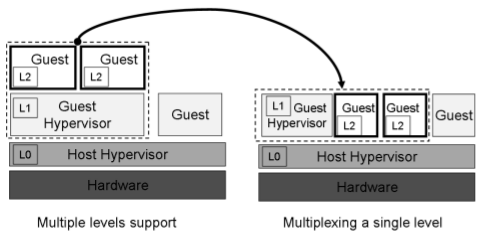
\includegraphics[width=4in]{images/turtles.png}
	\end{center}
	\caption{The Turtles hypervisor maintains logical nested virtualization, but
		in reality multiplexes all levels of nesting into $L_1$. (Figure courtesy
		of \cite{ref:turtles})}
	\label{fig:turtles-multiplex}
\end{figure*}

There are two difficult problems here that turtles provides a unique solution for.
The first involves page tables for the MMU.  In a nested model, virtual addresses for $L_2$
will need to be translated three times (first to physical addresses at $L_2$, then to $L_1$
addresses, and finally to $L_0$ addresses)
before they are readable by the hardware.  Modern MMUs provide support for virtualization
in the form of two distinct translation tables to make this process fast, but this is not
sufficient for more than one level of virtualization.  Furthermore, providing these
translation tables by emulating them in software is slow, particularly on updates,
for the reasons described above.  The paper's novel solution here is to use
\emph{multidimensional page tables}.  Essentially, each level keeps its own
shadowed page tables in software, but they are read-only.  On a page fault in $L_2$,
$L_0$ catches the trap and forwards it to $L_1$.  If $L_1$ also faults, $L_0$ allows
it to update its shadow table with the $L_2$-to-$L_1$ translation, but then applies
its tranlation for $L_1$ addresses to update the hardware table with the correct
$L_2$-to-$L_0$ translation before returning.  In this way, the hardware table at $L_0$
contains all the shadow tables above it compressed into a single table, so that
any MMU accesses can look up the correct translations directly from the hardware
without having to go through cascading levels of shadow tables first.  Turtles
also employs ``huge pages'' and Virtual Processor ID tags on page table entries
to ensure that page tables remain small and fast.

The second difficulty deals with device I/0.  Traditional approaches to this problem
involve either software emulation (which is slow), installing modified drivers in the
guest (which is not preferrable), or assigning devices to guests as they have need
of them (which is hard in the nested case).  Turtles uses something called
\emph{multi-level device assignment}, which is essentially an adaptation of the
multidimensional page table idea to the device I/O problem.  Modern chipsets
include a component called an IOMMU, which resides between the DMA and main memory
and performs translations just like the MMU does for the CPU.  By shadowing read-only
IOMMU translation tables at higher levels, and then compressing them into a single
hardware-level table, the DMA can avoid the same cascading translation issue that
would affect the MMU, thus making DMA I/O access very efficient.  For Memory-Mapped I/O
and Network Port I/O, address translation is not an issue, and so here techniques for
single-level device assignment are used without any penalty.

The Turtles paper provides an extensive evaluation section, with thorough experimentation
comparing performance of applications running on the native OS, a single-level VM, and the
Turtles two-level nested VM.  The authors measure and discuss performance on microbenchmarks,
I/O intensive workloads, and workloads that are designed to fault to the kernel constantly.
The paper also analyzes the success of multidimensional paging and multi-level device
assignment by testing these techniques against more traditional ways of handling these
problems.  In general, the Turtles hypervisor far outperforms any other approach to
nested virtualization considered, and is able to minimize the overhead of a second
level of virtualization to as low as 6-8\%, which is rather impressive.  No experiments
were conducted involving more than two nested levels of virtualization, although analysis
seemed to indicate that most of the additional overhead incurred by adding a second level
came from cache pollution and the overuse of privileged instructions where it was not
necessary.

\subsection{mClock: Handling Throughput Variability for Hypervisor IO Scheduling}
\label{sec:summaries/mclock}

The mClock paper \cite{ref:mclock} is not targeted at nested virtualization,
but further explores
the issue of fair I/O device assignment raised in the Turtles paper.  This turns
out to be a very difficult problem even in the single-level case, particularly
when applied to virtualization in the cloud, where networked devices are
often shared not just between VMs running on one host, but between many hosts
across the network.  In the interest of fairness, a good hypervisor will try to
share device throughput equally across its guests, but in the networked case, the
total amount of capacity to share may fluctuate due to traffic from other
networked clients.  Furthermore, many OSes run their own device access algorithms
above the hypervisor level to improve performance; for example, physical disk
accesses may be reordered by the kernel to take advantage of spatial locality
when moving the disk head.  These sorts of optimizations are often difficult
for the hypervisor to multiplex without loss of efficiency.

The mClock algorithm seeks to fairly schedule the device I/O of multiple guests,
while maintaining each guest's limit (maximum throughput requirement), reservation
(minimum requirement), and weight (proportional share of capacity relative to
other guests).  The algorithm uses a ``novel, lightweight'' tagging scheme to
achieve this despite fluctuation in total capacity.  Previous attempts to solve
this problem were not able to achieve both of these goals simultaneously.

\begin{figure}[t]
	\begin{center}
		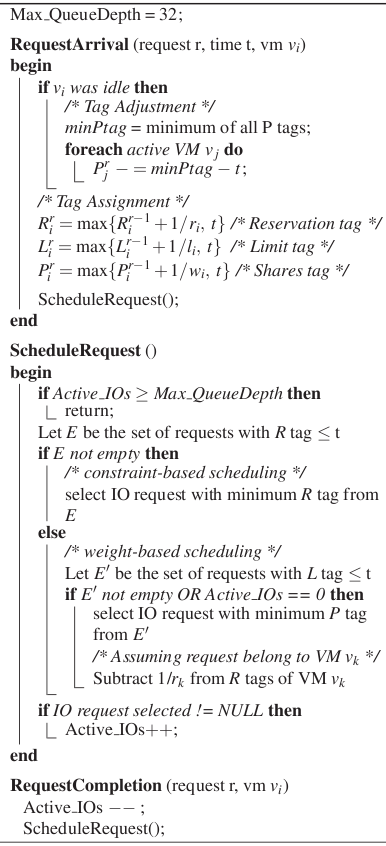
\includegraphics[width=2.5in]{images/mclock.png}
	\end{center}
	\caption{The mClock algorithm works by tagging requests with a tag for
		reservations, weights, and reservations, and then executing requests
		in order of their tags.  (Figure courtest of \cite{ref:mclock})}
	\label{fig:mclock-alg}
\end{figure}

The mClock algorithm (see Figure \ref{fig:mclock-alg}) works by assigning numerical tags to each
queued request.
Essentially, tags for VM $i$ with proportional weight $w_i$ will be spaced by $1/w_i$.
Requests will be executed in the order of their assigned tags, which ensures that
VM $i$ receieves his proportional share.  This approach requires a global clock
for tag assignment, so that idle clients remain synced with active ones and do not
amass ``idle credit'', thus gaining preferential treatment.  The tag for VM $i$ and
request $j$ is set as follows:

\[
	Tag(i, j) = max(curr~time, Tag(i, j-1) + 1/w_i)
\]

After the tagging, the request with the lowest tag will be scheduled.

In actuality, things are a little bit more complicated.  mClock maintains
3 types of tags and 3 global clocks, one each for reservations, weights,
and limits.  Each iteration of the algorithm is deemed to be
either a ``constraint-based phase'', in which some VM has not received
capacity above its reservation, or a ``weight-based phase'', in which the
next VM to be scheduled will be chosen by proportional share.  This is easily
determined after the tagging:  if any VM $i$ has request $j$ such that the
reservation tag $R(i, j)$ is less than the current time, than VM $i$ is currently
receiving less capacity than its reservation, and so the current phase is
constraint based.  Otherwise, the phase is weight-based, and so the algorithm
just picks a request with minimum weight tag $P(i, j)$ whose limit tag
$L(i, j)$ is also less than the current time (otherwise, VM $i$ is receiving
more capacity than its limit, and so it should not be scheduled).

The paper describes some further tweaks to the algorithm, such as allowing
a limited amount of idle credit to be saved up by idle VMs, or breaking ``large''
requests into a series of smaller requests to account for request latency
in the scheduler.  There's also a modifed dmClock algorithm for use with
a distributed storage system, which multiplexes VM requests fairly across multiple
storate servers.  Finally, there's a heuristic for setting reservations for
all VMs by default, so that no VM will be starved.

The authors include a lengthy evaluation of the performance of their algorithm.
They discuss many experiments involving different workloads and different combinations
of weights, limits, and reservations, and even test multiple types of devices
being assigned to analyze the effects of device latency and varying throughput.
Overall, mClock is extremely effective at meeting its guarantees for weights, limits,
and reservations when there is enough capacity to satisfy all requests, and
the algorithm degrades gracefully by sharing capacity proportionally when
the total capacity is insufficient.

The algorithm is successful at delivering on its guarantees despite contention,
which is important for ensuring VM isolation, and also has implications in the cloud,
where meeting quality of service guarantees determine financial success.

\subsection{Virtualize Everything but Time}
\label{sec:summaries/time}

The ``Virtualize Everything but Time'' paper \cite{ref:time} notes that accurate
timekeeping has become very important in today's computing systems, with
applications to everything from systems measurement and distributed database
consistency to high-speed trading and billing for cloud services.  However, 
timekeeping in a VM context is very difficult.  Historically, timekeeping
is accomplished using software clocks based on hardware oscillators, and
keeping the software clocks synchronized to an online
reference clock.  However, the synchronization algorithms used rely on
computing delays between timestamped packets, and the delay computation
turns out to be extremely unstable in a virtualized context, due mostly
to added latency during packet processing.

This paper does not really introduce a novel idea, but rather applies
an existing alternative solution for timekeeping to the virtualized context,
and then performs some rigorous experimentation to show that this solution
is better-suited.

In the hardware, there are a few oscillators that may be used as sources
for timekeeping.  Most systems today make use of the \emph{Time Stamp Counter}
(TSC), a high-resolution counter based on CPU cycles, and the
\emph{High Precision Event Timer} (HPET), which (ironically enough) has a
lower resolution than the TSC, and is slower to access as well.  The authors
mention hardware counters only because the technique currently used for timekeeping
in virtualized systems, Xen's Clocksource algorithm, relies on these two counters,
using the HPET for low-resolution ``ticks'', but interpolating between them using
the TSC.  However, this TSC data must be carefully adjusted before use, because
it is subject to drift based on a variety of other variables.

The focus of the paper is more on timekeeping synchronization algorithms.
The most popular contender in this arena is the \emph{Network Time Protocol} (NTP).
NTP is a feedback algorithm, which works by collecting and timestamping a series
of packets from a networked reference clock, computing clock error using
the reference timestamp-local timestamp pairings as data points, 
and updating the system clock accordingly.  Xen Clocksource makes use of NTP,
although it must be adapted to fit the virtualized context.  There are two
possibilities for this:  in Dependent Clocksource, \emph{dom0} runs an NTP
clock, and all guests running in \emph{domU} sync periodically to this NTP
clock and use Clocksource to interpolate between syncs.  Alternatively, there
is an Independent Clocksource paradigm in which each \emph{domU} guest runs their own
NTP clock.  The paper conducts evaluation of both paradigms, and argues
that neither is well-suited to the virtualized context.  Dependent Clocksource
exhibits cyclical sawtoothed drift because the Clocksource algorithm in
\emph{domU} does not have direct access to the TSC, and so cannot adjust
the NTP clock data intelligently.  Independent Clocksource is extremely
inefficient, but even worse, additional latencies incurred by contention for
network I/O tend to push the Clocksource feedback algorithm into instability,
so that large error can accumulate even across NTP synchronizations.

The authors instead endorse an alternative sync algorithm, \emph{RADClock}
(Robust Absolute and Difference Clock).  RADClock is a stateless, feed-forward
algorithm.  Like NTP, RADClock timestamps reference packets, but does so using
a ``raw'' clock based on hardware counters.  The raw clock's error is estimated
as before, but rather than using this data to update the clock (which would make
RADClock a feedback algorithm), the error is instead stored in memory, along
with some other clock parameters for the period of the counter and an offset
for the timescale being used.  When the clock is read, the time is adjusted
as
\[
	C(t) = Raw(t) * (ctr~period) + (offset) - error(t)
\]
RADClock adjusts equally well to either the dependent or equally dependent paradigm,
since no interpolation is needed to maintain the clock between syncs, as long
as all dependent clocks can look up accurate and up-to-date parameters.

The paper proceeds to rigorously evaluate the performance of Xen Clocksource
using NTP against RADClock, both in dependent and independent modes of
operation, and in a variety of different system conditions.  The conclusion
seems to be that RADClock is generally unaffected by the errors and
drift that plague clocksource (see Figure \ref{fig:time-eval}).
This is especially clear in a series of
experiments conducted involving VM migrations, where ``migration shock''
pushes the Independent Clocksource clock into a state of instability that
takes nearly 20 minutes to correct, while dependent RADClock converges
instantly.  Furthermore, the RADClock algorithm works equally well
regardless of the choice of underlying hardware counter, and is much
less affected by high contention for the network and system resources,
making it a better solution for the problem of timekeeping in the
context of virtualization.

\begin{figure*}[t]
	\caption{The RADClock algorithm consistently outperforms ntpd clocksource;
		here, the drift in clocksource is simply due to feedback from increased
		latency in the network. (Figure courtesy of \cite{ref:time})}
	\label{fig:time-eval}
	\begin{center}
		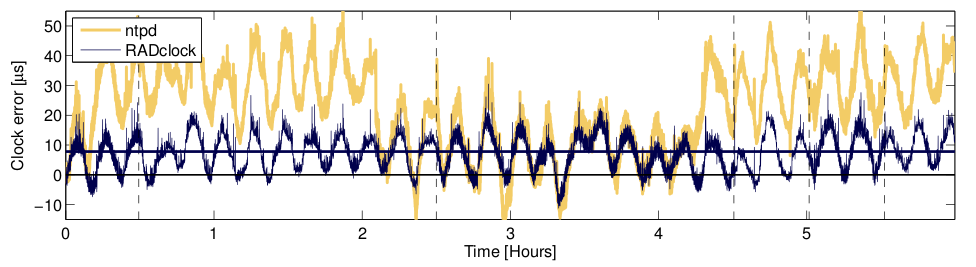
\includegraphics[width=6in]{images/time.png}
	\end{center}
\end{figure*}

\section{Paper Relationships}
\label{sec:relns}

As we surveyed this series of papers, we noticed that the literature
in this area seems to neatly classify itself by \emph{motivation}.
Many papers on virtualization come from the realm of academia, and these
are mostly characterized by a focus on clean abstractions and solutions
with good theoretical properties, such as fairness and strong isolation.
Many more papers, however, originate from corporate research at places
like Microsoft and HP Labs.  These papers seem much more interested
in providing fast, scalable solutions using commodity hardware and
software.  In our papers, we found a series of tensions which seemed
to be expressing this fundamental question of motivation.  We will
now turn our attention to these tensions, keeping in mind that the
Turtles and mClock papers share corporate authorship, while the
Denali and Time papers have originated in the realm of academia.

\subsection{Performance and Fairness}
\label{sec:relns/perf-fair}

The most obvious tension which surfaced in the literature was a question
of priority between performance and fairness.  Generally speaking, there is a trend
in corporate papers to be heavily concerned with speed and efficiency, while
academically-minded papers seem more focused on strong properties of isolation
and guarantees of fairness between VMs.  This should not be particularly surprising,
given the authorship; more efficient virtualization seems to be an easily reachable
step toward greater profit.  It is worth noting, however, that in the more recent
literature corporate papers seem to be taking note of the importance of fairness;
we will discuss this further in Section \ref{sec:relns/scale}.

Our papers are clearly divided by this metric:  Turtles is all about efficiency
and performance, often at the cost of fairness.  The problem seems
especially hard here because of the nested context.  It seems perfectly logical that if
a guest OS running in $L_2$ should only receive a fraction $\alpha$ of the resources allocated
to its host in $L_1$, which in turn should only receive a percentage $\beta$ of the machine's
total resources, then these two fractions should compound and our guest should end up with
$\alpha\beta$ of the total capacity available.  However, in reality Turtles multiplexes
all guests at all levels onto $L_0$, so in many ways the guest OS and its hypervisor will
be treated as siblings rather than a parent and child.  Multi-level device assignment
for Port I/O and Memory-mapped I/O is particularly agnostic to these concerns, because
it works exactly the same way as single-level device assignment, and so doesn't care whether
a guest runs at $L_1$ or $L_{100}$.  Furthermore, no experimentation at all is done to analyze
the effects of this model on fairness, and the authors even make the statement that this
is a secondary concern, and so they are content with a sort of best-effort.

On the other hand, Denali and mClock are all about prioritizing fairness.  The foundational
goal of the Denali isolation kernel is to ensure strong isolation between clients, so that
the behavior of any particular VM cannot in any way affect another.  And the whole point of
the mClock scheduling algorithm is to ensure that limits, reservations, and weights
are met fairly between VMs contending for a resource.  It should be noted that neither
of these papers particularly eschew performance as a worthy goal; rather, the view
here seems more to be that fast performance for a particular guest doesn't really
mean much if a malicious (or even just selfish neighbor) can somehow choke that VM
out and make it impossible to make progress.

The Time paper is somewhat agnostic to concerns of performance and fairness anyway,
since it deals more with the abstractions presented to client applications.  We
will turn to this next.

\subsection{Paravirtualization and Full Virtualization}
\label{sec:relns/para-full}

The second tension seems to arise between the paradigms of \emph{paravirtualization}
and \emph{full virtualization}, which were introduced in Section \ref{sec:background}.
Corporately-funded literature seems to have an eye more toward using as much
commodity software as possible here, for the sake of lower adoption costs, while
academic papers seem more willing to consider modifying client software in
appropriate situations.

The split here is pretty clear as well: Denali, Xen, and Time all consider
paravirtualization to be beneficial and even necessary in the right situations.
In Denali, the isolation kernel presents a modified and simplified hardware abstraction
to its clients, which cleverly allows for some big wins in efficiency and performance
as a side effect.  Xen claims that paravirtualization is necessary to ensure fairness
and prevent starvation in process and I/O scheduling; one could argue, however, that
this is no longer a concern due to the advent of newer virtualization-aware hardware
(see Section \ref{sec:relns/hard-emul}).  The Time paper goes a step further and claims that
even with the new hardware, making the guest OS aware of the virtualized context it
runs in is necessary to ensure the correctness of certain time-dependent applications!

In contrast, the Turtles project argues for full virtualization and unmodified guest
OSes and hypervisors.  In the paper, the argument for this goes back to the
motivating question of efficiency, though it was unclear to us why paravirtualization
would have any negative impact here.  But it seems also that for any sort of large-scale
commercial deployment of server virtualization technology, the ability to use commodity
guests would be crucial in order to make adoption easy, and we consider this to also
be a likely factor influencing the design choice.

The mClock paper doesn't really fit into these two classifications, since it mostly
deals with the interactions between the hypervisor and its devices, rather than the hypervisor
and its guests.  However, the paper does mention that one of the reasons this disk
scheduling problem is so difficult is because guest OSes have their own algorithms
for efficient disk scheduling, which generally don't play nice with each other.  If it
were possible to modify the guest OS to disable these algorithms, so that the hypervisor
could handle all disk scheduling decision, the difficulty of this problem could likely
be reduced.

\subsection{Hardware Support and Software Emulation}
\label{sec:relns/hard-emul}

The ``tension'' between hardware support for virtualization and the use of software
emulation is perhaps better just described as a paradigm shift.  It seems
that over the last decade virtualization-friendly hardware has become commonplace
and inexpensive.  When the Xen and Denali papers were written, there was no real
alternative, and so everything had to be done through slow, inefficient software emulation.
But when hardware manufacturers began to produce virtualization-enabled chipsets
like the x86, this problem essentially disappeared overnight, and it has largely
remained out-of-scope for most of the intervening decade.

However, the question of software emulation may need to be re-examined as virtualization
research moves foward.  While hardware-enabled approaches are clearly much faster
than any attempt to do all the work in software, it seems that it just may not be possible to do
everything at the hardware level.  The Turtles project is a perfect example of this - there
is no hardware support for nested levels of virtualization, and so a lot of cleverness
is required to be able to compensate in the software without an unacceptable performance
penalty.  We have essentially been sent back to where single-level virtualization
solutions were a decade ago.  Some of the future work mentioned in this paper involved
examining ways to provide architectural support for nested virtualization, but although
we are somewhat skeptical that this will prove fruitful.  Attempting to provide
support for an unbounded number of levels of nesting with finite hardware does
not seem like it would be particularly successful.  It will be interesting to
see what direction this sort of work takes in the future, and whether hardware
designers will rise to the challenge of nested virtualization.

\subsection{Scalability and the Cloud}
\label{sec:relns/scale}

The final tension we wish to consider is the question of scalability.  We have observed
that there is a commercial interest in developing super-scalable server virtualization,
largely because it has found such a unique niche with the market growth of cloud computing
and infrastructure-as-a-service (IAAS).  While academic research is not uninterested in the question
of scale or the cloud use case, we do not feel that they are as much of a driving factor in this realm.

We can observe this trend in the papers we have been discussing.  The Turtles paper presents
the motivation for nested virtualization using the argument of its suitability for
infrastructure-as-a-service, as the two are essentially made for each other.  The mClock paper,
although it does not particularly market itself
for scalability, is motivated by the cloud-enabled scenario of many virtualized clients
needing to schedule the use of a shared network disk.  Furthermore, the guarantees mClock
makes about fairness, reservations, and proportional share are especially important
in this scenario, as they allow IAAS providers to keep service-level agreements with
their clients.  We find this particularly interesting, as it seems to indicate
that in the cloud, fairness and performance may find themselves on equal footing in
terms of importance (see Section \ref{sec:relns/perf-fair}).

Interestingly, the Denali paper also has a particular eye to scalability, and a large
portion of the evaluations section is devoted to demonstrating that the isolation kernel
performs well even when supporting over 10,000 VMs.  However, even in Denali, scalability
is just one goal amongst many, and the paper does not really consider applications
to cloud computing, being several years too early.

The Time paper does not really consider the question of scalability at all, being
somwhat orthogonal to the problem of accurate timekeeping on a single VM.  The paper
does point out that there are scalability benefits to the dependent RADClock algorithm,
as each VM no longer needs to send out synchronization packets on the network, but can
depend on the hypervisor to do this for all VMs that it hosts.  However, this is 
in many ways just an added bonus, and is not really a motivational argument for the paper.

\section{Conclusion}
\label{sec:conclusion}

Having examined the recent literature along these four axes of tension, it is our belief
that a clear trend has emerged in virtualization.  We believe that as cloud computing and
IAAS continue to take off, research in this area will continue to trend toward what
is both popular and financially successful.  We expect that the majority of virtualization
research will continue in the direction of full virtualization over paravirtualization,
and that the cloud-computing/IAAS scenario will become the driving use case.
However, we think that as a result of this, fairness and performance will no longer be
competing ends, but will in fact become equal players.  This will be necessary in order
for cloud providers to meet their SLAs to their consumers, and we believe fair-scheduling
and resource-isolation research will move from its place in the shadows to the forefront
of both corporate and academic research.

As to the question of hardware support versus software emulation, we believe that as
new directions like nested virtualization are explored, some sort of hybrid approach
will continue to be needed.  However, we do not expect the status quo of fast hardware-enabled
virtualization to be shaken up in the general case; it seems that performance is too critical
in the driving cloud-based use cases, and we would be surprised to see nested virtualization
(or any other software-hybrid approach) gaining momentum here anytime soon.

Cynical though it may be, we feel that a lot of the interesting problems in virtualization
have already been solved, at least from an academic perspective.  So much of the recent
literature seems to be in the direction of just making things more efficient and more
reliable for the sake of the commercialized cloud.  We have stopped asking the question,
``can we do crazy thing $x$?'', and now are only asking ``how much faster can we make $x$ work?''
and ``how can we make $x$ work with fewer resources?''
This is certainly an important part of the research process for any area, but it is ostensibly
less exciting than the ground-breaking work that was going on earlier in the decade.

Of course, we cannot say with any certainty that there is not some new, groundbreaking discovery
just waiting to be made around the corner.  Such a discovery could revitalize the field
and take virtualization off into all sorts of new and exciting directions.  But we do feel that
the way the problem has been framed makes it unlikely that such a new discovery could shift
the focus away from cloud-based server virtualization.  With so much focus on making the problem
fit into the market niche, such a new discovery would have to be truly monumental indeed -
monumental enough that no one could possibly predict it.

\begin{thebibliography}{10}

{\footnotesize

\bibitem{ref:xen}
	P. Barham, B. Dragovic, K. Fraser, S. Hand, T. Harris, A. Ho, R. Neugebauer,
	I. Pratt, and A. Warfield.  Xen and the Art of Virtualization.  In {\it Proc. of
	the 19\textsuperscript{th} ACM Symp. on Operating Systems Principles}, 2003.

\bibitem{ref:denali}
	A. Whitaker, M. Shaw, and S. Gribble.  Scale and Performance in the Denali Isolation
	Kernel.  In {\it Proc. of the 5\textsuperscript{th} Symp. on Operating Systems
	Desgin \& Implementation}, 2002.

\bibitem{ref:turtles}
	M. Ben-Yehuda, M. Day, Z. Dubitzky, M. Factor, N. Har'El, A. Gordon, A. Liguori,
	O. Wasserman and B. Yassour.  The Turtles Project: Design and Implementation
	of Nested Virtualization.  In {\it Proc. of the 9\textsuperscript{th}
   USENIX Symp. on Operating Systems Design \& Implementation}, 2010.

\bibitem{ref:mclock}
	A. Gulati, A. Merchant, and P. Varman.  mClock: Handling Throughput Variability
	for Hypervisor IO Scheduling.  In {\it Proc. of the 9\textsuperscript{th}
   USENIX Symp. on Operating Systems Design \& Implementation}, 2010.

\bibitem{ref:time}
	T. Broomhead, L. Cremean, J. Ridoux, and D. Veitch.  Virtualize Everything but
	Time.  In {\it Proc. of the 9\textsuperscript{th}
   USENIX Symp. on Operating Systems Design \& Implementation}, 2010.

}

\end{thebibliography}

\end{document}
